\chapter{LaTeX Hints}
\label{sec:latexhints}

This chapter contains hints on writing LaTeX.
It focuses on minimal examples, which can be directly adapted to the content

\section{Handling of paragraphs}

\begin{ltgexample}
One sentence per line.
This rule is important for the usage of version control systems.
A new line is generated with a blank line.
As you would do in Word:
New paragraphs are generated by pressing enter.
In LaTeX, this does not lead to a new paragraph as LaTeX joins subsequent lines.
To start a new paragraph, press enter twice.
This leads to an empty line.
In word, there is the functionality to press shift and enter.
This leads to a hard line break.
The text starts at the beginning of a new line.
In LaTeX, you can do that by using two backslashes (\textbackslash\textbackslash).
\\
Running text seldom needs a hard line break.

Please do \textit{not} use two backslashes for new paragraphs.
For instance, this sentence belongs to the same paragraph, whereas the last one started a new one.
Andrew Stacey gives a long motivation for that in the section \enquote{Line Wrapping} of his \href{https://loopspace.mathforge.org/HowDidIDoThat/TeX/VCS/#section.3}{\emph{Document Revision System}}\footnote{\url{https://loopspace.mathforge.org/HowDidIDoThat/TeX/VCS/}}.
\end{ltgexample}

Once the text is final, single paragraphs can be polished.
If the last line of a paragraph holds only a word or two, or is nearly full, let TeX set the paragraph one line shorter or longer: write \texttt{\textbackslash looseness=-1} (or \texttt{=1}) as the first thing in that paragraph.
TeX resets \texttt{\textbackslash looseness} at the end of every paragraph, so only that one paragraph is affected.
With LuaLaTeX, a lone short word as the last line is avoided automatically (package impnattypo).

\section{Notes separated from the text}

The package mindflow enables writing down notes and annotations in a way so that they are separated from the main text.

\begin{ltgexample}
\begin{mindflow}
This is a small note.
\end{mindflow}
\end{ltgexample}

\section{Handling TODOs}

\begin{ltgexample}
\textmarker{Marked text.}
\end{ltgexample}

With \verb1\textmarker1, only the text color is changed, since this also works well for individual words.

\begin{ltgexample}
\textcomment{Marked text.}{A comment on it.}
\end{ltgexample}

\begin{ltgexample}
\hl{Highlighted in yellow.}
Provided indirectly by the pdfcomment package (via soulpos).
\end{ltgexample}

\begin{ltgexample}
\modified{Manual marking for text that has been changed since the last version.}
\end{ltgexample}

\begin{ltgexample}
This is some text.
\change{FL1: text adjusted}{Changed text}.
\end{ltgexample}

\begin{ltgexample}
Here is a comment\sidecomment{Comment}.
\end{ltgexample}

\begin{ltgexample}
\todo{A lot of text still needs to be produced here}
\end{ltgexample}

\section{Hyphenation}

\LaTeX{} automatically hyphenates words.
When using \href{https://ctan.org/pkg/microtype}{microtype}, there should be fewer hyphenations than in other settings.
You might still need to tweak the hyphenation.
Here are some hints:

\begin{ltgexample}
In case you write \enquote{application-specific}, then the word will only be hyphenated at the dash.
You can also insert \verb1\allowbreak{}1 into the word, as in applica\allowbreak{}tion-specific, but this is much more effort.

You can now write words containing hyphens which are hyphenated at other places in the word.
For that, write \verb1"=1 instead of \verb1-1, as in application"=specific.
This is enabled by an additional configuration of the babel package.
\end{ltgexample}

\section{Typesetting Units}

\begin{ltgexample}
Numbers can be written plain text (such as 100), by using the \href{https://ctan.org/pkg/siunitx}{siunitx} package as follows:
\SI{100}{\km\per\hour},
or by using plain \LaTeX{} (and math mode):
$100 \frac{\mathit{km}}{h}$.
\end{ltgexample}

\begin{ltgexample}
\SI{5}{\percent} of \SI{10}{kg}
\end{ltgexample}

\begin{ltgexample}
Numbers are automatically grouped: \num{123456}.
\end{ltgexample}

\section{Surrounding Text by Quotes}

\begin{ltgexample}
Please use the \enquote{enquote command} to quote something.
Quoting with "`quote"' or ``quote'' also works.

\end{ltgexample}

\section{Zref-clever examples}
\label{sec:ex:cref}

Demonstration of zref-clever: Zcref (short for zcref[S]) at the beginning of a sentence, zcref in all other cases.

\begin{figure}
  \centering
  \includegraphics[width=.75\linewidth]{example-image-a}
  \caption{Example figure for zcref demo}
  \label{fig:ex:cref}
\end{figure}

\begin{table}
  \caption{Example table for zcref demo}
  \label{tab:ex:cref}
  \centering
  \begin{tabular}{ll}
    \toprule
    Heading1 & Heading2 \\
    \midrule
    One      & Two      \\
    Three    & Four     \\
    \bottomrule
  \end{tabular}
\end{table}

\begin{ltgexample}
\Zcref{fig:ex:cref} shows a simple fact, although \zcref{fig:ex:cref} could also show something else.

\Zcref{tab:ex:cref} shows a simple fact, although \zcref{tab:ex:cref} could also show something else.

\Zcref{sec:ex:cref} shows a simple fact, although \zcref{sec:ex:cref} could also show something else.
\end{ltgexample}

\section{Formulas and Equations}

\begin{ltgexample}
Equations $f(x)=x$ inside the text can be provided.
\end{ltgexample}

A list with all available mathematical symbols is provided at \url{http://texdoc.net/pkg/symbols-a4}.

\begin{ltgexample}
As an example, the set of natural numbers is given by $\mathbb{N}$.
\end{ltgexample}

For the documentation of editing mathematical formulas, read the package documentation of \texttt{amsmath}\footnote{\url{http://texdoc.net/pkg/amsmath}}.

\Zcref{eq:test} is numbered and can be referenced in the text:
\begin{ltgexample}
\begin{align}
  \label{eq:test}
  x = y
\end{align}
\end{ltgexample}

The following equation is not numbered because of using \texttt{\textbackslash align*} as environment.
\begin{ltgexample}
\begin{align*}
  x = y
\end{align*}
\end{ltgexample}

The template offers \verb+\abs+ to enable the bars to scale well at the absolute value:
\begin{ltgexample}
$\abs{X}$.
\end{ltgexample}

The documentation available at \url{http://www.ctan.org/tex-archive/help/Catalogue/entries/voss-mathmode.html} provides more details about mathematical environments.

\section{Figures}

\begin{ltgexample}
\Zcref{fig:label} shows something interesting.

\begin{figure}
  \centering
  \includegraphics[width=.8\linewidth]{example-image-golden}
  \caption[Simple Figure]{
    Simple Figure.
    Based on \citet{mwe}.
  }
  \label{fig:label}
\end{figure}
\end{ltgexample}

Photos in JPEG or PNG format are included the same way, as shown in \zcref{fig:jpg}.

\begin{ltgexample}
\begin{figure}
  \centering
  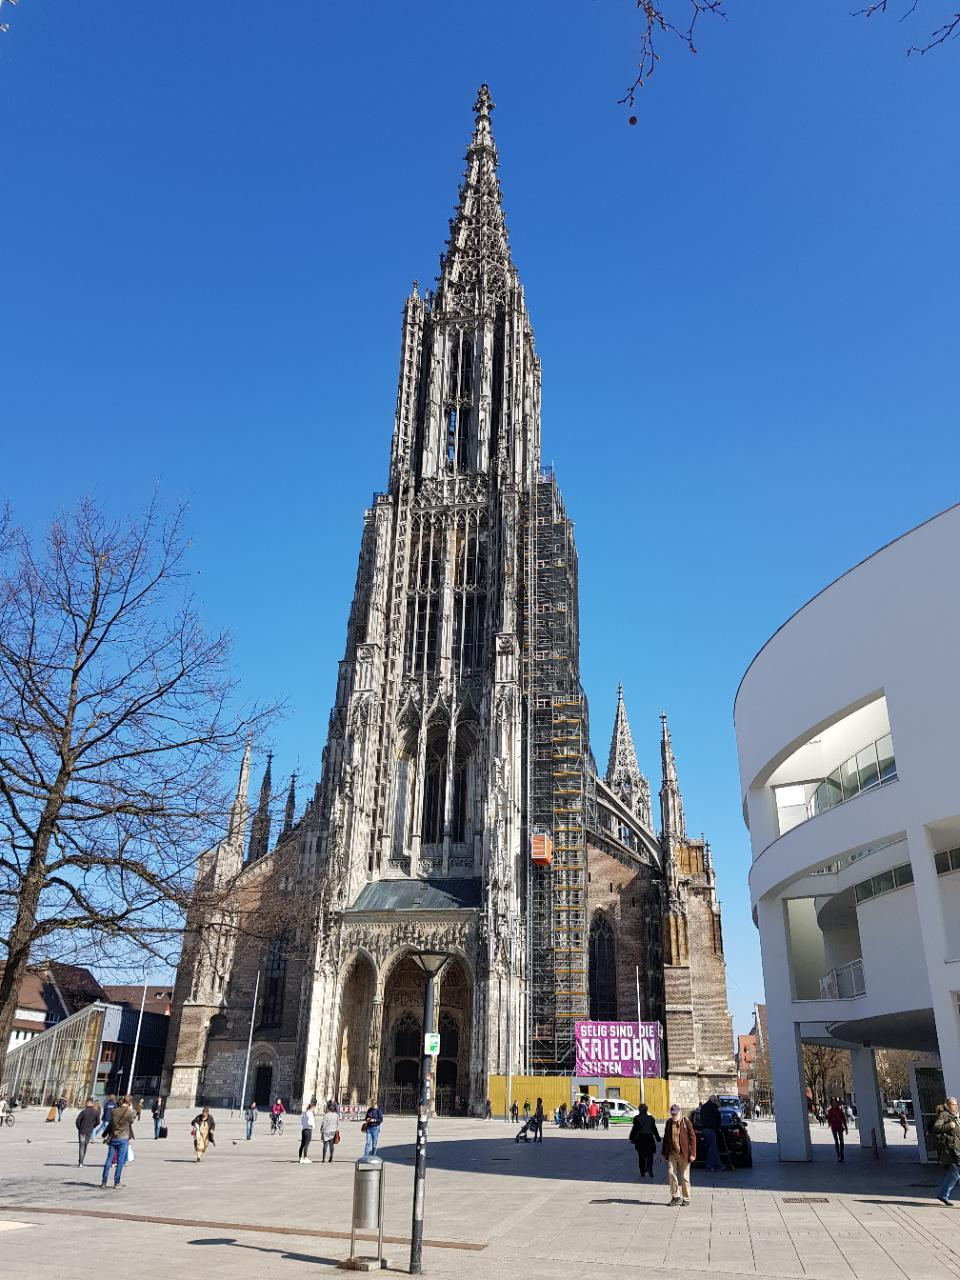
\includegraphics[width=.5\linewidth]{figures/ulm-minster.jpg}
  \caption{Ulm Minster. Photo: wkrauth, CC0, via Wikimedia Commons.}
  \label{fig:jpg}
\end{figure}
\end{ltgexample}

\section{Sub Figures}

An example of two sub figures is shown in \zcref{fig:two_sub_figures}.

\begin{ltgexample}
\begin{figure}[!b]
  \centering
  \subfloat[Case I]{\includegraphics[width=.4\linewidth]{example-image-a}%
    \label{fig:first_case}}
  \hfil
  \subfloat[Case II]{\includegraphics[width=.4\linewidth]{example-image-b}%
    \label{fig:second_case}}
  \caption{Example figure with two sub figures.}
  \label{fig:two_sub_figures}
\end{figure}
\end{ltgexample}

\section{Figures with tikz}

The \href{https://ctan.org/pkg/pgf}{tikz} package creates graphics programmatically.
This package generates grids and other regular structures.

\begin{ltgexample}
\begin{figure}[ht]
  \centering
  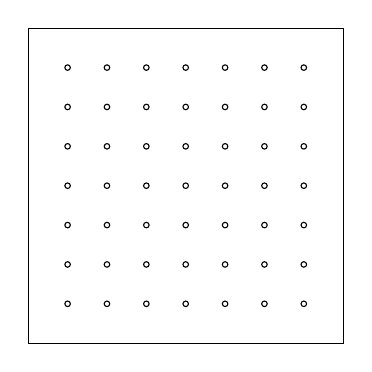
\begin{tikzpicture}
    \draw(0,0) rectangle (4,4);
    \foreach \x in {0.5,1,1.5,2,2.5,3,3.5}
    \foreach \y in {0.5,1,1.5,2,2.5,3,3.5}
    \draw(\x,\y) circle (1pt);
  \end{tikzpicture}
  \caption{A regular grid generated easily with two for loops.}\label{fig:tikz_example}
\end{figure}
\end{ltgexample}

\section{Plots with pgfplots}

The \href{https://ctan.org/pkg/pgfplots}{pgfplots} package plots functions directly in \LaTeX{}, similar to MATLAB or gnuplot.
Some visual examples are available in the package documentation\footnote{\url{http://texdoc.net/pkg/pgfplots}}.

\begin{ltgexample}
\begin{figure}[ht]
  \centering
  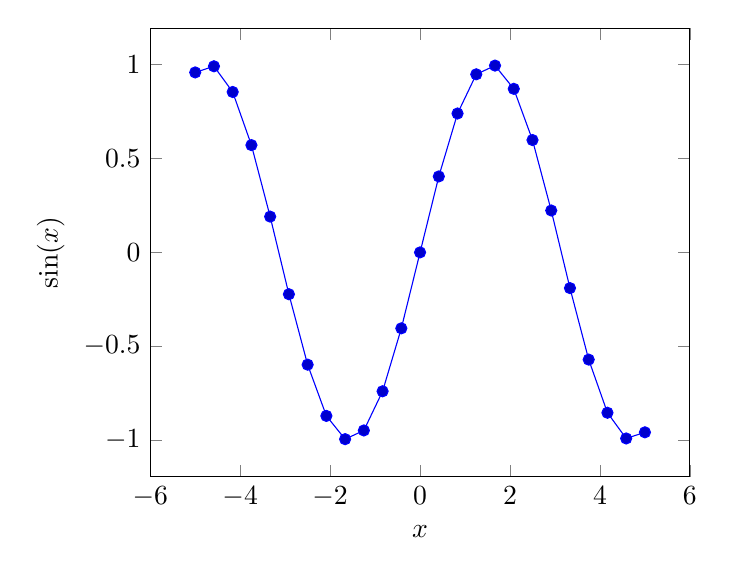
\begin{tikzpicture}
    \begin{axis}[xlabel=$x$, ylabel=$\sin(x)$]
      \addplot {sin(deg(x))};  % Plot the sine function
    \end{axis}
  \end{tikzpicture}
  \caption{Plot of $\sin(x)$ directly inside the figure environment with pgfplots.}
  \label{fig:pgfplots_example}
\end{figure}
\end{ltgexample}

Coordinates can also be given explicitly instead of as a function:
\begin{ltgexample}
\begin{figure}[ht]
  \centering
  \begin{tikzpicture}
    \begin{axis}[xlabel=$x$, ylabel=$y$]
      \addplot coordinates {(0,0) (1,1) (2,4) (3,9)};  % Plot explicit coordinates
    \end{axis}
  \end{tikzpicture}
  \caption{Explicit coordinates plotted with pgfplots.}
  \label{fig:pgfplots_coords}
\end{figure}
\end{ltgexample}

\section{UML diagrams}

UML diagrams can be written as text next to the \LaTeX{} source and are typeset in the fonts of the document.
\href{https://ctan.org/pkg/metauml}{MetaUML} draws class, component, and further diagrams.
It is MetaPost code, which \texttt{lualatex} runs itself via the \href{https://ctan.org/pkg/luamplib}{luamplib} package; no further tools are needed.
Thus, the MetaUML diagrams are shown only when compiling with \texttt{lualatex}.
The \href{https://ctan.org/pkg/pgf-umlsd}{pgf-umlsd} package draws sequence diagrams with TikZ and works with every engine.
A comparison of the packages for UML diagrams is given at \url{https://github.com/latextemplates/gadr-latex-packages/blob/main/uml-diagrams.md}.

\ifluatex
  \begin{ltgexample}
  \begin{figure}
    \centering
    \sffamily
    \begin{mplibcode}
      input metauml;
      beginfig(1);
      Class.Driver("Driver")()();
      Class.Car("Car")("+model: String")("+drive()");
      Class.Wheel("Wheel")()();
      Class.Person("Person")()();
      % distances between the boxes in PostScript points (1/72 inch)
      leftToRight(70)(Driver, Car, Wheel);
      topToBottom(50)(Car, Person);
      drawObjects(Driver, Car, Wheel, Person);
      link(association)(Driver.e -- Car.w);
      item(iAssoc)("drives >")(obj.s = .5[Driver.e, Car.w]);
      % the diamond is drawn at the end of the path
      link(composition)(Wheel.w -- Car.e);
      item(iAssoc)("have 4 >")(obj.s = .5[Car.e, Wheel.w]);
      link(association)(Car.s -- Person.n);
      item(iAssoc)("< owns")(obj.w = .5[Car.s, Person.n] + (5, 0));
      endfig;
    \end{mplibcode}
    \caption{Class diagram drawn with MetaUML}
    \label{fig:uml-class}
  \end{figure}
  \end{ltgexample}

  \begin{ltgexample}
  \begin{figure}
    \centering
    \sffamily
    \begin{mplibcode}
      input metauml;
      beginfig(1);
      Component.Client("Client")();
      Component.Server("Server")();
      % MetaUML has no automatic layout: each object is placed relative to another one;
      % here, the left edge of Server is 140 PostScript points (1/72 inch, about 5 cm) right of the right edge of Client
      Server.w = Client.e + (140, 0);
      drawObjects(Client, Server);
      % the interface: Server provides it (ball), Client requires it (socket)
      pair iface;
      iface = .5[Client.e, Server.w];
      link(providedInterface)(Server.w -- iface);
      link(requiredInterface)(Client.e -- iface);
      item(iAssoc)("API")(obj.s = iface + (0, 8));
      endfig;
    \end{mplibcode}
    \caption{Component diagram drawn with MetaUML}
    \label{fig:uml-component}
  \end{figure}
  \end{ltgexample}
\fi

\begin{ltgexample}
\begin{figure}
  \centering
  \sffamily
  \begin{sequencediagram}
    \newthread{client}{Client}
    % [3]: horizontal gap (in cm) to the box of the previous instance; the default (0.2) leaves no room for the message labels
    \newinst[3]{server}{Server}
    \begin{call}{client}{request()}{server}{response}
    \end{call}
  \end{sequencediagram}
  \caption{Sequence diagram drawn with pgf-umlsd}
  \label{fig:uml-sequence}
\end{figure}
\end{ltgexample}

\section{Tables}

\begin{ltgexample}
\begin{table}
  \caption{Simple Table}
  \label{tab:simple}
  \centering
  \begin{tabular}{ll}
    \toprule
    Heading1 & Heading2 \\
    \midrule
    One      & Two      \\
    Three    & Four     \\
    \bottomrule
  \end{tabular}
\end{table}
\end{ltgexample}

A table caption goes above the table (\verb|\caption| before the \verb|tabular|), a figure caption below the figure.

Rows and cells can be colored with \verb|\rowcolor| and \verb|\cellcolor| from the \href{https://ctan.org/pkg/colortbl}{colortbl} package, which \href{https://ctan.org/pkg/xcolor}{xcolor} loads with its option \verb|table|.

\begin{ltgexample}
\begin{table}
  \caption{Table with colored cells}
  \label{tab:colored}
  \centering
  \begin{tabular}{ll}
    \toprule
    \rowcolor{gray!20}
    Test & Result                   \\
    \midrule
    A    & \cellcolor{green!20}pass \\
    B    & \cellcolor{red!20}fail   \\
    \bottomrule
  \end{tabular}
\end{table}
\end{ltgexample}

A \verb|\footnote| inside a floating table is lost.
Use \verb|\tablefootnote| from the \href{https://ctan.org/pkg/tablefootnote}{tablefootnote} package instead: it is set as a normal footnote at the bottom of the page.
If the notes should appear directly below the table instead (common in journals), use the \href{https://ctan.org/pkg/threeparttable}{threeparttable} package.

\begin{ltgexample}
\begin{table}
  \caption{Table with a footnote}
  \label{tab:footnote}
  \centering
  \begin{tabular}{ll}
    \toprule
    Heading1 & Heading2\tablefootnote{A footnote inside a table.} \\
    \midrule
    One      & Two                                                \\
    \bottomrule
  \end{tabular}
\end{table}
\end{ltgexample}

\begin{ltgexample}
% Adapted from https://tex.stackexchange.com/a/468994/9075
\begin{table}
  \caption{Table with diagonal line}
  \label{tab:diag}
  \begin{center}
    \begin{tabular}{|l|c|c|}
      \hline
      \diagbox{Row}{Column} & A & B \\
      \hline
      1                     & x & y \\
      \hline
    \end{tabular}
  \end{center}
\end{table}
\end{ltgexample}


\section{Tables spanning multiple pages}

The \href{https://ctan.org/pkg/longtable}{longtable} package typesets tables that automatically break across page boundaries.
The header (\verb+\endhead+) and footer (\verb+\endfoot+) rows are repeated on every page; once enough rows are added, the table spans more than one page on its own.

\begin{ltgexample}
\begin{longtable}{|l|l|l|}
  \caption{A sample long table.}\label{tab:long} \\
  \hline
  \multicolumn{1}{|c|}{\textbf{First column}} & \multicolumn{1}{c|}{\textbf{Second column}} & \multicolumn{1}{c|}{\textbf{Third column}} \\ \hline
  \endfirsthead

  \multicolumn{3}{c}{{\bfseries \tablename\ \thetable{} -- continued from previous page}} \\
  \hline
  \multicolumn{1}{|c|}{\textbf{First column}} & \multicolumn{1}{c|}{\textbf{Second column}} & \multicolumn{1}{c|}{\textbf{Third column}} \\ \hline
  \endhead

  \hline \multicolumn{3}{|r|}{{Continued on next page}} \\ \hline
  \endfoot

  \hline\hline
  \endlastfoot

  A & BC & D \\
  A & BC & D \\
  A & BC & D \\
  A & BC & D \\
  A & BC & D \\
  A & BC & D \\
  A & BC & D \\
  A & BC & D \\
  A & BC & D \\
  A & BC & D \\
  A & BC & D \\
  A & BC & D \\
\end{longtable}
\end{ltgexample}

% The main file loads either the minted or the listings package
\ifdefined\inputminted
  \section{Source Code}

The \href{https://github.com/gpoore/minted}{minted} package highlights listings properly.
It uses the \href{http://pygments.org/}{pygments} library, which in turn requires Python.

\begin{ltgexample}
\Zcref{lst:XML} shows source code written in XML.
\refline{line:comment} contains a comment.

\begin{listing}[htbp]
  \begin{minted}[linenos=true,escapeinside=||]{xml}
<listing name="example">
  <!-- comment --> |\labelline{line:comment}|
  <content>not interesting</content>
</listing>
\end{minted}
  \caption{Example XML listing using minted}
  \label{lst:XML}
\end{listing}
\end{ltgexample}

One can also typeset JSON as shown in \zcref{lst:flJSON}.

\begin{ltgexample}
\begin{listing}[htbp]
  \begin{minted}[linenos=true,escapeinside=||]{json}
{
  key: "value"
}
\end{minted}
  \caption{Example JSON listing using minted}
  \label{lst:flJSON}
\end{listing}
\end{ltgexample}

Java is also possible as shown in \zcref{lst:flJava}.

\begin{ltgexample}
\begin{listing}[htbp]
  \begin{minted}[linenos=true,escapeinside=||]{java}
public class Hello {
    public static void main (String[] args) {
        System.out.println("Hello World!");
    }
}
\end{minted}
  \caption{Java code rendered using minted}
  \label{lst:flJava}
\end{listing}
\end{ltgexample}

Listings longer than the remaining space continue on the next page if they are \emph{not} floating.
A floating listing is always placed on a single page.
Thus, use \verb+\captionof{listing}+ instead of the \verb+listing+ environment.
\Zcref{lst:long} spans multiple pages.

\begin{minted}[linenos=true]{java}
public class Squares {

    /** Returns the square of 1. */
    public int square1() {
        return 1 * 1;
    }

    /** Returns the square of 2. */
    public int square2() {
        return 2 * 2;
    }

    /** Returns the square of 3. */
    public int square3() {
        return 3 * 3;
    }

    /** Returns the square of 4. */
    public int square4() {
        return 4 * 4;
    }

    /** Returns the square of 5. */
    public int square5() {
        return 5 * 5;
    }

    /** Returns the square of 6. */
    public int square6() {
        return 6 * 6;
    }

    /** Returns the square of 7. */
    public int square7() {
        return 7 * 7;
    }

    /** Returns the square of 8. */
    public int square8() {
        return 8 * 8;
    }

    /** Returns the square of 9. */
    public int square9() {
        return 9 * 9;
    }

    /** Returns the square of 10. */
    public int square10() {
        return 10 * 10;
    }

    /** Returns the square of 11. */
    public int square11() {
        return 11 * 11;
    }

    /** Returns the square of 12. */
    public int square12() {
        return 12 * 12;
    }

    public static void main(String[] args) {
        System.out.println(new Squares().square12());
    }
}
\end{minted}
\captionof{listing}{Long Java listing spanning multiple pages}
\label{lst:long}

\else
  \section{Source Code}

\begin{ltgexample}
\Zcref{lst:XML} shows source code written in XML.
\Zcref{line:comment} contains a comment.

\begin{lstlisting}[
  language=XML,
  caption={Example XML Listing},
  label={lst:XML}]
<listing name="example">
  <!-- comment --> (* \label{line:comment} *)
  <content>not interesting</content>
</listing>
\end{lstlisting}
\end{ltgexample}

One can also add \verb+float+ as parameter to have the listing floating.
\Zcref{lst:flXML} shows the floating listing.

\begin{ltgexample}
\begin{lstlisting}[
  % one can adjust spacing here if required
  % aboveskip=2.5\baselineskip,
  % belowskip=-.8\baselineskip,
  float,
  language=XML,
  caption={Example XML listing -- placed as floating figure},
  label={lst:flXML}]
<listing name="example">
  Floating
</listing>
\end{lstlisting}
\end{ltgexample}

One can also typeset JSON as shown in \zcref{lst:json}.

\begin{ltgexample}
\begin{lstlisting}[
  float,
  language=json,
  caption={Example JSON listing -- placed as floating figure},
  label={lst:json}]
{
  key: "value"
}
\end{lstlisting}
\end{ltgexample}

Java is also possible as shown in \zcref{lst:java}.

\begin{ltgexample}
\begin{lstlisting}[
  caption={Example Java listing},
  label=lst:java,
  language=Java,
  float]
public class Hello {
    public static void main (String[] args) {
        System.out.println("Hello World!");
    }
}
\end{lstlisting}
\end{ltgexample}

Listings longer than the remaining space continue on the next page if they are \emph{not} floating.
A floating listing is always placed on a single page.
\Zcref{lst:long} spans multiple pages.

\begin{lstlisting}[
  language=Java,
  caption={Long Java listing spanning multiple pages},
  label={lst:long}]
public class Squares {

    /** Returns the square of 1. */
    public int square1() {
        return 1 * 1;
    }

    /** Returns the square of 2. */
    public int square2() {
        return 2 * 2;
    }

    /** Returns the square of 3. */
    public int square3() {
        return 3 * 3;
    }

    /** Returns the square of 4. */
    public int square4() {
        return 4 * 4;
    }

    /** Returns the square of 5. */
    public int square5() {
        return 5 * 5;
    }

    /** Returns the square of 6. */
    public int square6() {
        return 6 * 6;
    }

    /** Returns the square of 7. */
    public int square7() {
        return 7 * 7;
    }

    /** Returns the square of 8. */
    public int square8() {
        return 8 * 8;
    }

    /** Returns the square of 9. */
    public int square9() {
        return 9 * 9;
    }

    /** Returns the square of 10. */
    public int square10() {
        return 10 * 10;
    }

    /** Returns the square of 11. */
    public int square11() {
        return 11 * 11;
    }

    /** Returns the square of 12. */
    public int square12() {
        return 12 * 12;
    }

    public static void main(String[] args) {
        System.out.println(new Squares().square12());
    }
}
\end{lstlisting}

\fi

\section{Itemization}

One can list items as follows:

\begin{ltgexample}
\begin{itemize}
  \item Item One
  \item Item Two
\end{itemize}
\end{ltgexample}

With the package paralist, one can create itemizations with lesser spacing:

\begin{ltgexample}
\begin{compactitem}
  \item Item One
  \item Item Two
\end{compactitem}
\end{ltgexample}

One can enumerate items as follows:

\begin{ltgexample}
\begin{enumerate}
  \item Item One
  \item Item Two
\end{enumerate}
\end{ltgexample}

With the package paralist, one can create enumerations with lesser spacing:

\begin{ltgexample}
\begin{compactenum}
  \item Item One
  \item Item Two
\end{compactenum}
\end{ltgexample}

With paralist, one can even have all items typeset after each other and have them clean in the TeX document:

\begin{ltgexample}
\begin{inparaenum}
  \item The first item,
  \item the second item, and
  \item the third item appear in one line.
\end{inparaenum}
\end{ltgexample}

\section{Writing in Markdown}\label{sec:markdown}

\ifluatex
  If you are new to \LaTeX{}, you can start by writing your text in Markdown using the \href{https://ctan.org/pkg/markdown}{markdown} package.
  \LaTeX{} then takes care of the typesetting.
  Markdown and \LaTeX{} can be mixed:
  \Zcref{tbl:markdown} is written in Markdown and referenced from \LaTeX{}.
  A whole chapter can be written in a separate Markdown file included by \verb|\markdownInput|, as \zcref{sec:markdown-file} shows.
  The \href{https://github.com/latextemplates/markdown-latex-quickstart}{markdown-latex-quickstart} shows a complete document written in Markdown.

  \begin{ltgexample}
  \begin{markdown}
Text can be *emphasized* or **bold**, and `code` is set in a monospaced font.
A citation looks like this [@mwe], and here is a footnote.^[This is an inline footnote.]

- first point
- second point
  - sub-point

1) firstly
2) secondly

| Right | Left | Centered |
|------:|:-----|:--------:|
|    12 | 12   |    12    |
|   123 | 123  |   123    |

: A table written in Markdown {#tbl:markdown}

<#tbl:markdown> shows a table with caption.
Its identifier `{#tbl:markdown}` is referenced by `<#tbl:markdown>`.
\end{markdown}
  \end{ltgexample}
\else
  This example requires \hologo{LuaLaTeX}.
  Compile the document with \hologo{LuaLaTeX} to see it.
\fi

\section{Abbreviations}

With \verb+\gls{...}+, you can enter abbreviations: the first time you call it, the long form is used.
When reusing \verb+\gls{..}+ the short form is automatically displayed.
The abbreviation is also automatically inserted in the abbreviation list.
With \verb+\glspl{...}+ the plural form is used.
If you want the short form to appear directly at the first use, you can use \verb+\glsunset{..}+ to mark an abbreviation as already used.
The opposite is achieved with \verb+\glsreset{..}+.

Abbreviations are defined in \verb+\content\ausarbeitung.tex+ by means of \verb+\newacronym{...}{...}{...}+.

More information at: \url{https://ctan.org/pkg/bib2gls}.

\begin{ltgexample}
At the first pass, the \gls{er} was 5.
At the second pass was \gls{er} 3.
The plural form can be seen here: \glspl{er}.
To demonstrate what the list of abbreviations looks like for longer description texts, \glspl{rdbms} must be mentioned here.

\gls{dante} is a local \TeX\ user group.
The German-speaking local \TeX\ user group is \gls{dante}.
A \gls{gp} is a medical doctor.
I went to my surgery to see the \gls{gp}.
\end{ltgexample}

\todo{Include difference between acronym and abbreviation - \url{https://tex.stackexchange.com/a/154566/9075}}

\section{Other Features}

\begin{ltgexample}
The words \enquote{workflow} and \enquote{dwarflike} can be copied from the PDF and pasted to a text file.
\end{ltgexample}

\begin{ltgexample}
The symbol for powerset is now correct: $\powerset$ and not a Weierstrass p ($\wp$).

$\powerset({1,2,3})$
\end{ltgexample}

\begin{ltgexample}
Brackets work as designed:
<test>
One can also input backticks in verbatim text: \verb|`test`|.
\end{ltgexample}

Acronyms can be typeset in running text with \verb+\initialism+, which sets them as small caps that blend into the surrounding lowercase text. It is the lightweight alternative to the full acronym and glossary management (\verb+\gls+, with an automatic list of abbreviations) provided by the thesis variants: \verb+\initialism+ only typesets the acronym and does not add it to any list. The macro and the ready-made acronyms (\verb+\OMG+, \verb+\BPEL+, \verb+\BPMN+, \verb+\UML+) are defined in \texttt{commands.tex}, where you can add your own.

\begin{ltgexample}
The \UML is maintained by the \OMG; related standards include \BPEL and \BPMN.
Any acronym can be set inline with \initialism{REST} or \initialism{HTTP}.
\end{ltgexample}


\section{Zref-vario examples}
\label{sec:ex:vref}

Demonstration of zref-vario: zvref[S] at the beginning of a sentence, zvref in all other cases.

\begin{ltgexample}
\zvref[S]{fig:ex:cref} shows a simple fact, although \zvref{fig:ex:cref} could also show something else.

\zvref[S]{tab:ex:cref} shows a simple fact, although \zvref{tab:ex:cref} could also show something else.

\zvref[S]{sec:ex:cref} shows a simple fact, although \zvref{sec:ex:cref} could also show something else.
\end{ltgexample}

\section{Citations}

When referencing something from the bibliography file, it will automatically appear in the references section.
If a reference is not cited, it is not appearing there.

\begin{ltgexample}
Standard case: Citing indirectly citing something~\cite{mwe}.
In case one wants to name the author: \textcite{mwe} shows a minimal \LaTeX{} example.
\end{ltgexample}

Note that \texttt{\textbackslash textcite\{mwe\}} prints both the author and the reference to the bibliography entry.

A thesis is cited like any other work: a master's thesis~\cite{Shannon1940} or a doctoral thesis~\cite{Nash1950}.
The entry types \texttt{@MastersThesis} and \texttt{@PhdThesis} are labeled in the document language (\enquote{MA thesis} or \enquote{Masterarbeit}, \enquote{PhD thesis} or \enquote{Diss.}).
For a Bachelor's thesis, use \texttt{@Thesis} with \texttt{type = \{bathesis\}}; for a Diplomarbeit, \texttt{type = \{Diplomarbeit\}} is printed as is.

Remember that you have to call \texttt{biber main-english} to generate the bibliography data for \texttt{lualatex}.
You will need to run \texttt{lualatex} twice so that the page numbers are up to date.


In the bibliography, use \texttt{\textbackslash textsuperscript} for \enquote{st}, \enquote{nd}, \ldots:
E.g., \enquote{The 2\textsuperscript{nd} conference on examples}.
When you use \href{https://www.jabref.org}{JabRef}, you can use the cleanup command to achieve that.
See \url{https://help.jabref.org/en/CleanupEntries} for an overview of the cleanup functionality.

\section{Miscellaneous Examples}
\label{ssec:example}

Reference test: \Zcref{ssec:example}, \zcref{fig:Abbildung} and \zcref{alg:example}.

\begin{ltgexample}
Checkmark: \dingcheck.
Crossmark: \dingcross.
\end{ltgexample}

\begin{figure}
  \missingfigure{}
  \caption{Figure}
  \label{fig:Abbildung}
\end{figure}

\begin{landscape}
  \begin{figure}
    \missingfigure{}
    \caption{Rotated figure}
    \label{fig:AbbildungGedreht}
  \end{figure}
\end{landscape}

\subsection{Algorithms}

\begin{algorithm}
  \caption{$algo$}
  \label{alg:example}
  \begin{algorithmic}[1]
    \State $a \gets 0$
    \State State 2\label{alg1:state2}
  \end{algorithmic}
\end{algorithm}

\begin{algorithm}
  \caption{Algorithm 2}
  \label{alg:example2}
  \begin{algorithmic}[1]
    \State $a \gets 0$
    \State State 2\label{alg2:state2}
  \end{algorithmic}
\end{algorithm}

\Zcref{alg:example} has already shown an algorithm.
Test of line referencing: line~\ref{alg1:state2} (\zcref{alg:example}) and line~\ref{alg2:state2} (\zcref{alg:example2}).

\subsection{Definitions}
\begin{definition}[Title]
  \label{def:def1}
  Definition Text
\end{definition}

\Zcref{def:def1} shows \ldots

\subsection{Enumerations}

\begin{enumerate}[label=\alph*)]
  \item a
  \item b
  \item c
  \item d
\end{enumerate}

Equivalent to paralist's inparaenum:
\begin{enumerate*}[label=\alph*)]
  \item a
  \item b
  \item c
  \item d
\end{enumerate*}

\begin{description}
  \item[first] First
  \item[second] Second
  \item[third] Third
\end{description}

\begin{description}
  \item[\texttt{first}] First
  \item[\texttt{second}] Second
  \item[\texttt{third}] Third
\end{description}

%works only if package enumitem is loaded
\begin{description}[font=\ttfamily]
  \item[first] First
  \item[second] Second
  \item[third] Third
\end{description}

\begin{description}[style=unboxed]
  \item[first label with a long description text breaking over one line. Enabled by the enumitem package] First
  \item[second] Second
  \item[third] Third
\end{description}

\begin{Description}
  \item[first label with a long description text breaking over one line. Defined in the template] First
  \item[second] Second
  \item[third] Third
\end{Description}

\begin{itemize}
  \item First
  \item Second
  \item Third
\end{itemize}

The optional parameter changes the marker that is prepended.
See \url{http://www.weinelt.de/latex/item.html}.
\begin{itemize}
  \item[A] First
  \item[B] Second
  \item[C] Third
\end{itemize}

Incorrect use of the optional parameter as follows:
\begin{itemize}
  \item[first] First
  \item[second] Second
  \item[third] Third
\end{itemize}
Note that, when \texttt{enumitem} is loaded, this behaves differently than with \texttt{paralist}.

\subsection{The fquote environment}

\begin{fquote}[T.\ Scientist]
  The program will be finished by next Friday.
\end{fquote}

\begin{gfquote}{T.\ Scientist}
  The program will be finished by next Friday.
\end{gfquote}
